\documentclass[a4paper,11pt]{article}
\usepackage[utf8]{inputenc}
\usepackage{microtype} %improves justification
\usepackage{graphicx}
\usepackage{csquotes}
\usepackage{wrapfig}
\usepackage{enumitem}
\usepackage{fancyhdr} % header
\usepackage{amsmath} % math formulas
\usepackage{index}
\usepackage[backend=biber, sorting=none]{biblatex}
\addbibresource{library.bib}
\usepackage[portuguese]{babel}
\usepackage[paper=a4paper, top=2.5cm, bottom=2.5cm, left=2.5cm, right=2.5cm]{geometry}
%\usepackage{indentfirst}
\usepackage{bm}
\newcommand{\bfitDelta}{\bm{\mathit{\Delta}}}
\usepackage{caption}
% \numberwithin{equation}{section}
\usepackage{blindtext}

\newcommand\tabitem{\setlength{\itemindent}{1cm}}
\newcommand\tabtabitem{\setlength{\itemindent}{2cm}}

\usepackage{ulem}
\usepackage{times}   % Times New Roman

\pagestyle{fancy}
\fancyhf{}
\rfoot{\thepage}


\setlength\parindent{24pt}
\newcommand\tab[1][0.8cm]{\hspace*{#1}}

\renewcommand{\headrulewidth}{0pt}
%\newcommand\notab{\setlength{\parindent}{0cm}}
%\textbf{NEGRITO}
%\textit{ITÁLICO}
%\underline{SUBLINHADO}
\usepackage{afterpage}

\usepackage{appendix}

\usepackage{chngcntr}
\counterwithin{figure}{section} % NUMERAÇÃO DAS FIGURAS CONSOANTE CAPÍTULO
\counterwithin{table}{section}  % // TABELAS



\begin{document}

\renewcommand{\listfigurename}{Índice de figuras}

\renewcommand{\listtablename}{Índice de tabelas}
    
%\DeclareNameAlias{sortname}{family-given}
%\DeclareNameAlias{default}{family-given}

\begin{titlepage}
\newgeometry{top=1.5cm, bottom=2cm}


   \begin{center}
        
\includegraphics[width=0.3\textwidth]{0 - Capa/EEUMfinal.png}\\
        \vspace{0.2cm}
        \textbf{Licenciatura em Engenharia Eletrónica e de Computadores}
       \vfill
        
       \textbf{\Large{Caloiros De Elite: \textit{Space Invaders}}}\\
       \vspace{0.2cm}
       \textbf{\large{Complementos de Programação de Computadores}}\\

       \vfill
   

        Ano Letivo de 2021/2022\\
        \vspace{0.2pt}
        a101168, Afonso Gomes\\
        a101170, Christian Garcia\\
        \vspace{0.2pt}
        Guimarães, maio de 2022  \vspace{0.8cm}
   \end{center}        % CAPA
\end{titlepage}     % TÍTULO



\pagebreak


\newgeometry{top=2.5cm, left=2.5cm, right=2.5 cm, bottom=2.5cm}
\pagenumbering{roman}


\setcounter{secnumdepth}{-1}
\section{Resumo}
% \markboth{Resumo}{Resumo}

\tab Este trabalho consiste numa explicação extensa da criação do jogo \textbf{"Caloiros de Elite"}, inspirado no jogo \textbf{"Space Invaders"}, desenvolvido pela \textit{Taito Corporation} \cite{spaceInv}.  \par
\vspace{8pt}

     % 2º parágrafo
     
\vspace{8pt}

     % 3º parágrafo
\vspace{40pt}


\pagebreak

\pagebreak


\renewcommand{\contentsname}{Índice}        % ÍNDICE
\tableofcontents
\addcontentsline{toc}{section}{Índice}

\vspace{40pt}
\listoffigures

\vspace{40pt}
\listoftables

\pagebreak


\setcounter{secnumdepth}{3}


\section{Introdução}\label{Intro}

\pagenumbering{arabic}
\setcounter{page}{1}
\tab 

\vspace{8pt}

Grande parte da população que programa as ferramentas de \textit{software} que utilizamos na atualidade viu-se motivada pelos videojogos da geração dos 70s, 80s e 90s. \textit{PACMAN, Tetris} e \textit{Space Invaders} são alguns exemplos deste fenómeno que cada dia influencia mais jovens e adultos a mergulharem no imenso banco de dados que conhecemos como a Internet e começarem a programar.

\vspace{8pt}

O objetivo deste trabalho é desenvolver um jogo, inspirado por \textit{Space Invaders}, utilizando as diferentes ferramentas fornecidas pela linguagem de programação C++, nomeadamente, a utilização de OPP (\textit{Object Oriented Programming}), leitura e alteração de ficheiros, entre outros.

\vspace{8pt}

O trabalho distribui-se em diferentes temáticas, sendo estas a descrição geral do jogo (natureza e estratégias utilizadas para a sua implementação),  arquitetura do sistema (são apresentados, de forma geral, os módulos utilizados e a estrutura do jogo) e finalmente a implementação do mesmo, sendo neste último onde se vai expor ao pormenor cada uma das soluções utilizadas no presente problema.

\pagebreak

\section{Descrição do Problema}

\vspace{8pt}

\tab
\textit{Caloiros de Elite} é um jogo do subgénero \textit{Shoot'em Up}, onde o jogador, representado de forma predeterminada pelo símbolo do curso de Eletrónica, tem de acabar com diferentes ondas de inimigos, representados pelos outros cursos de engenharia, e \textit{bosses}, representados pelos departamentos de Medicina e Ciências e pela própria Universidade do Minho. 

\vspace{8pt}

O jogo tem duas modalidades principais: o modo "história", onde se tem de sobreviver o ataque de diferentes inimigos ao longo de três níveis diferentes, e o modo \textit{"Endless"}, em que procura-se obter a máxima pontuação possível enquanto se sobrevive e acaba com inimigos gerados de forma aleatória, infinitamente.

\vspace{8pt}

A primeira modalidade, o modo história, consta de quatro níveis de dificuldade, transformando o jogo numa experiência mais desafiante, sendo o último, "\textit{Hardcore}", o mais difícil deles todos, com só uma vida. Ao longo dos três níveis que conformam esta modalidade, o jogador tem de sobreviver e derrotar aos diferentes \textit{bosses} mencionados anteriormente, acabando por se enfrentar a uma versão final da Universidade de Minho, como inimigo definitivo do jogo. O modo \textit{Endless}, em contraste, permite ao jogador uma experiência mais casual, sem perder a natureza desafiante que forma parte intrínseca do jogo (e da vida universitária). Neste, o jogador enfrenta ondas infinitas de inimigos e \textit{bosses}, na tentativa de sobreviver o máximo tempo possível e acabar com a maior quantidade de inimigos, resultando numa maior pontuação final.

\vspace{8pt}

Além da mecânica geral do jogo, este também permite a personalização da nave do jogador, como resultado da realização de certos desafios. Os prémios recompensam maioritariamente a habilidade do jogador e/ou tempo de jogo. Estes dados todos (pontuações máximas, prémios obtidos, estatísticas) ficam salvos no fim de cada experiência e podem ser visualizados em espaços determinados para o efeito (\textit{Hall of Fame}, \textit{Trophies}, \textit{Stats}...)

\vspace{8pt}

Para conseguir criar esta experiência de jogo, é necessário recorrer à OOP, sendo que a maioria dos elementos pode e deve ser representada como objetos, com atributos e métodos. Desta forma, conseguimos simplificar o código, iterando funções por entidades semelhantes.

\vspace{8pt}

Tendo em consideração a dificuldade do projeto, além das estratégias mencionadas previamente, é necessário a utilização do paradigma \textit{"Divide and Conquer"}, solucionando problemas de menor dimensão e combinando os resultados obtidos para atingir um objetivo final.

\pagebreak

\section{Arquitetura do Sistema}

\vspace{8pt}


O programa “Caloiros de Elite” através do ponto de vista do utilizador:

\begin{itemize}
    \item Menu principal: O utilizador escolhe de entre várias opções o que deseja fazer
    \tabitem
    \item \textit{Play}: opção principal do menu que se subdivide em 3 outras opções:
    \item \textit{New Game}: o utilizador opta entre 3 \textit{slots} distintos para guardar o jogo atual. Após a seleção são mostradas 4 dificuldades distintas para o modo história\textit{ (easy,normal,hard e hardcore)} nas quais variam a probabilidade dos inimigos dispararem, a vida dos \textit{bosses} e, no modo \textit{hardcore} as vidas visto que nesta dificuldade o jogador apenas tem 1 vida.

    \item \textit{Load Game}: o jogador escolhe entre 3 \textit{slots}, previamente inicializados na opção \textit{New Game}, e continua o jogo presente no \textit{slot} selecionado (com a excepção da dificuldade \textit{hardcore}).

    \item   \textit{Endless} : é pedido ao utilizador para inserir um nome que aparece em tempo real com a fonte utilizada ao longo do trabalho. Em seguida começa o jogo desde o início com 2 \textit{bosses} (um \textit{miniboss} e o \textit{boss} principal que contém uma barra de vida exibida no topo do ecrã). Este modo é infinito sendo que o objetivo é conseguir a maior pontuação possível.

    \item  \textit{Highscores}: são exibidos os \textit{scores }mais altos, em ordem decrescente de cima para baixo, obtidos no modo \textit{endless} e o nome de quem obteve tal pontuação, nome esse que é inserido quando \textit{endless} é inicializado.
    
    \item \textit{Trophies}: são mostrados os diferentes troféus adquiridos após a conclusão de certos desafios. 
<<<<<<< HEAD
<<<<<<< HEAD
<<<<<<< HEAD
    \item \textit{Settings}: opção onde o utilizador pode alterar o programa a seu gosto.
    \item  \textit{Costumization}: são exibidos vários nomes de curso que o utilizador pode optar para trocar a \textit{Skin} atual da nave, o que influencia os inimigos exibidos (não há inimigos iguais à nave).
    \item  \textit{Technical settings}: a resolução da janela e nível do som podem ser alterados através desta opção.
=======
    
    \item \textit{Settings}: 
    
>>>>>>> 850b8d194ad84a18eabc31ad02d1bb4b2fd62c4c
=======
    
    \item \textit{Settings}: 
    
>>>>>>> 850b8d194ad84a18eabc31ad02d1bb4b2fd62c4c
=======
    
    \item \textit{Settings}: 
    
>>>>>>> 850b8d194ad84a18eabc31ad02d1bb4b2fd62c4c
    \item \textit{Credits}: pode-se ver os nomes dos criadores do jogo. 
    
\end{itemize}
	    
      

        
                 
          
   
       
     
            
              
         
            
         
        
        
   
    
	
    

    









\begin{tabbing}
    
\end{tabbing}
O jogo, em nível de estrutura, pode ser divido em "experiência de jogo", gestão de dados, interface de utilizador e aspetos extras, como apresentado na figura \ref{fig:GameModulesDiagram}, sendo que esta organização não representa de forma direta a própria infraestrutura do código, mas os módulos ou elementos lógicos que compõem o todo que conforma o presente trabalho.

\vspace{8pt}

\begin{figure}[!ht]
    \centering
    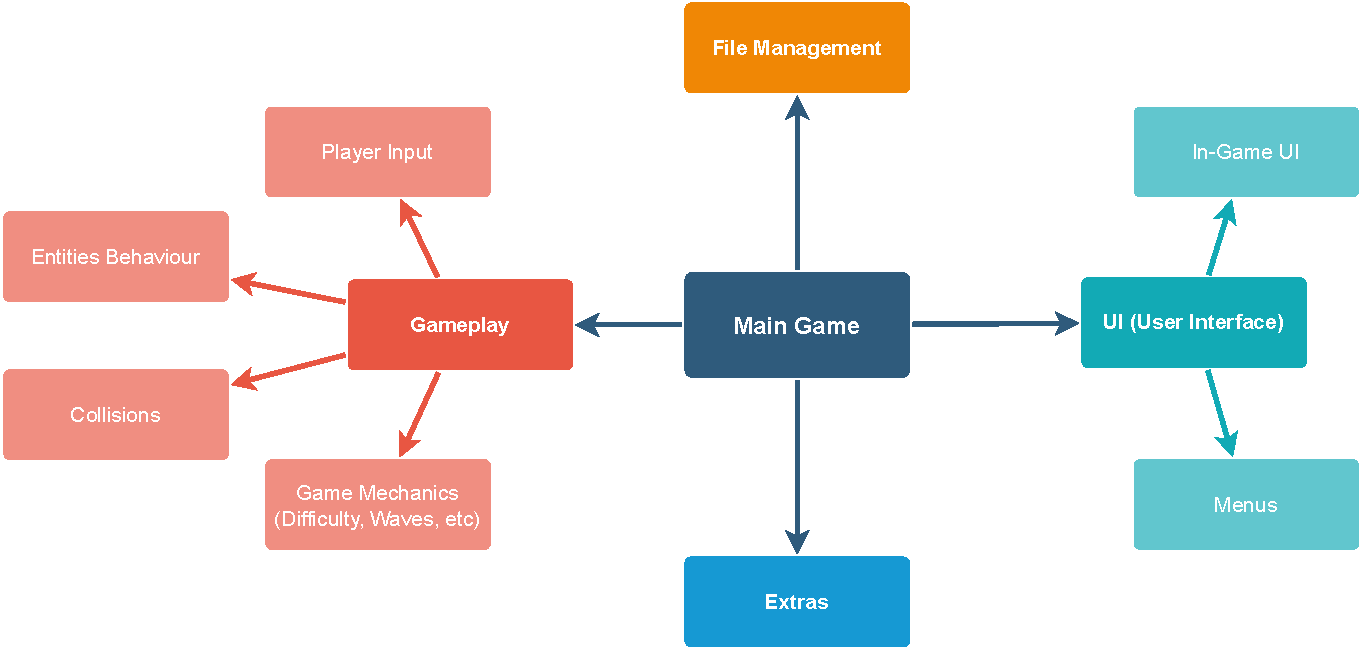
\includegraphics[scale = 0.60]{2 - Esquemas/GameModulesDiagram.pdf}
    \caption{Diagrama de blocos no desenvolvimento do jogo}
    \label{fig:GameModulesDiagram}
\end{figure}

\vspace{8pt}

O código só utiliza a linha lógica da estrutura apresentada, sendo que soluciona certos problemas que formam parte de "membros" do sistema organizacional em classes que representam maioritariamente membros diferentes, com fins de "simplificar" ou "reutilizar" código.

\vspace{8pt}

\subsection*{\textit{Gameplay}}

\vspace{8pt}

O \textit{Gameplay} vê-se refletido na classe \textit{Game}, sendo que esta controla todo aquilo referente aos elementos de uma experiência de jogo (comportamento das diferentes entidades, registo de pontuação se necessário, tratamento de colisões, entre outros elementos designados ao \textit{Gameplay} previamente). Algumas entidades requerem certo grau de complexidade, resultando na sua categorização exclusiva como "objetos do jogo", classe \textit{Objects}, engendrando as classes \textit{Player, Bullets, Enemies} e \textit{Bosses} (Figura \ref{fig:ClassGameplay}). No início de cada experiência de jogo, cria-se um objeto do tipo \textit{Gameplay}, criando este um objeto da classe \textit{Player} e, de forma dinâmica, variedade de objetos das outras subclasses de \textit{Objects}, conforme o jogo se desenvolve.

\vspace{8pt}

\begin{figure}[!ht]
    \centering
    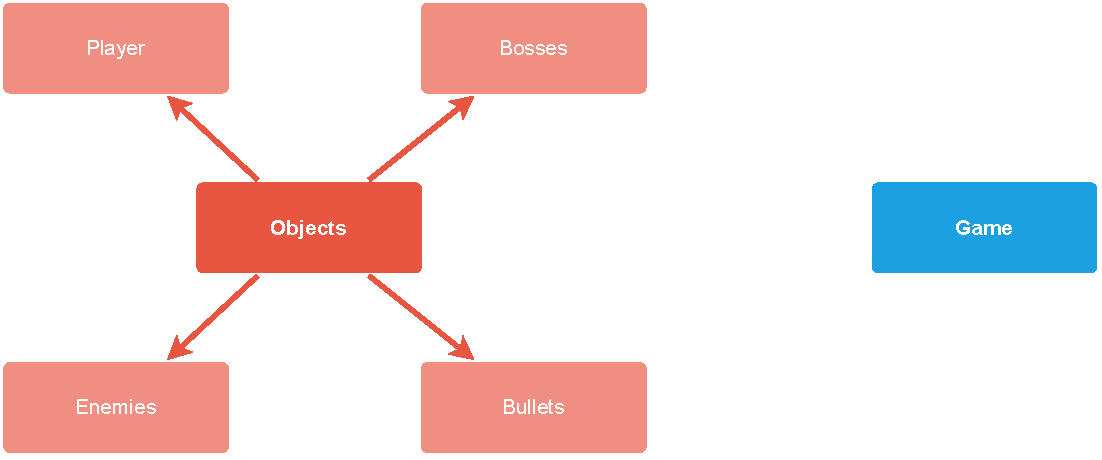
\includegraphics[scale = 0.60]{2 - Esquemas/ClassGameplay.pdf}
    \caption{Diagrama de blocos da distribuição e estrutura do módulo \textit{Gameplay}}
    \label{fig:ClassGameplay}
\end{figure}

\vspace{8pt}

\subsection*{UI - \textit{User Interface}}

\vspace{8pt}

Embora alguns elementos da UI estão presentes na classe \textit{Game}, nomeadamente, aqueles que têm relação com a \textit{In-Game UI}, a maior parte está representada na classe\dots \textit{Menu}, sendo esta a responsável por gerir e apresentar os \textit{menus} que permitem a visualização de estatísticas e prémios ou a configuração previa a uma experiência de jogo (\textit{skins}, dificuldade e modalidade).


\vspace{8pt}

\subsection*{\textit{File Management}}
O \textit{File Management} ocorre maioritariamente no menu onde são carregadas as estatísticas do jogo bem como os \textit{Highscores}, troféus e \textit{Skins} desbloqueadas. Toda a informação previamente mencionada é gravada num ficheiro no final de cada partida. Existe também algum \textit{File Management} nas opções \textit{New Game} e \textit{Load Game} onde são guardadas e carregadas as estatísticas do jogo atual, contudo, quando a dificuldade é \textit{Hardcore} não há qualquer carregamento do jogo atual.


\vspace{8pt}

\subsection*{Extras}

\vspace{8pt}


\pagebreak

\section{Implementação do Jogo}

\vspace{8pt}

\tab

"Caloiros de Elite" 

\vspace{8pt}

\subsection{Representação do Estado do Jogo}
\pagebreak

\subsection{Inicialização do Estado do Jogo}
\pagebreak

\subsection{Visualização do Estado do Jogo}
\pagebreak

\subsection{Mudança de estado/movimento do Jogador}
\pagebreak

\subsection{Salvar e Restaurar Jogo}
\pagebreak

\subsection{Final da Execução}
\tab Este projeto não tem um fim definido, apenas acaba quando o utilizador fecha a janela do jogo. Sendo assim focar-nos-emos no fim da sessão, ou seja, quando o jogador morre ou conclui o modo história. Quando o utilizador morre no modo história em qualquer dificuldade, o jogo tem em conta vários critérios:
\begin{itemize}
    \tabitem
    \item Número de inimigos mortos;
    \item Número de \textit{Bosses} eliminados;
    \item Se o jogador concluiu com sucesso ou não o modo história, e a dificuldade em que estava;
\end{itemize}
É depois atualizado o ficheiro das estatísticas com estes dados. Se o jogo estiver numa dificuldade diferente de \textit{Hardcore} é também gravado o nível onde o \textit{Player} se encontrava antes de morrer podendo este ser carregado mais tarde. 
\begin{tabbing}
    
\end{tabbing}
Caso seja \textit{Endless} o \textit{Highscore} é guardado bem como se houve ou não a destruição de um

\pagebreak

\tab Neste subcapítulo serão abordadas figuras, tabelas, equações e listas numeradas/não numeradas.

\subsubsection{Figuras}

\tab A figura \ref{fig:exemplo} é um exemplo da introdução de figuras em \LaTeX:

\begin{figure}[!ht]
    \centering
    \caption{Legenda da figura}
    \label{fig:exemplo}
\end{figure}


\subsubsection{Tabelas}

\tab Na tabela apresenta-se um exemplo de uma tabela em \LaTeX:

\subsubsection{Equações}

\tab Na equação \ref{eq:conservaçãomassaenergia} apresenta-se um exemplo de uma tabela em \LaTeX:

\begin{equation}\label{eq:conservaçãomassaenergia}
    E = m \cdot c^{2}
\end{equation}

\subsubsection{Listas}

\tab Apresente-se agora um exemplo de uma lista numerada:

\begin{enumerate}
    \tabitem
    \item item 1;
    \item item 2.
\end{enumerate}

Relativamente a listas não numeradas:

\begin{itemize}
    \tabitem
    \item item 1;
    \item item 2.
\end{itemize}

\pagebreak


\section{Conclusões e Perspetivas do Trabalho}

\tab Ao longo do trabalho foram-nos surgindo vários desafios e problemas que,com muito empenho e pesquisa, conseguimos resolver. Podémos também ter muita liberdade criativa visto que o tema base não nos restringiu de alguma forma, dando nos assim a liberdade para utilizar outras ferramentas para desenhar os sprites de todas as entidadades do jogo. \tab
    
Após a realização deste trabalho, conseguimos concluir que as classes lecionadas ao longo do semestre são realmente importantes na linguagem de C++, pois permitem uma melhor organização do código facilitando o trabalho do programador.\tab 

Por fim, em jeito de conclusão, pode dizer-se que este trabalho foi concluído com sucesso, pois conseguimos focar todos os pontos essenciais para a total conclusão do trabalho. Apesar de concluído com sucesso, é importante referir que ao longo de todo o processo de resolução, principalmente na fase de implementação e modulação, surgiram algumas dúvidas, dúvidas essas que felizmente não foram uma barreira que impediu a concretização deste trabalho. Contudo, houve certas funções que gostaríamos de ter implementado que acabaram por não ser concluídas, nomeadamente as \textit{technical settings}. Esta função não influencia nada na execução do jogo então de forma a não prejudicar a parte mais essencial do projeto, decidimos que esta seria a melhor opção.



\pagebreak






\printbibliography[title={Referências Bibliográficas}]


\pagebreak





\appendix

\section{Bibliografia}

\tab \Blindtext

\pagebreak

\end{document}
